\documentclass[letterpaper,12pt]{article}
\usepackage[utf8]{inputenc}
\usepackage{fullpage}
\usepackage{courier}
\usepackage[margin=0.75in]{geometry}
\usepackage{listings}
\usepackage{color}
\usepackage{graphicx}
\usepackage[width=5in]{caption}
\usepackage{hyphenat}
\usepackage{hyperref}
\usepackage{float}
\usepackage{multirow}

% Format a sectionless paragraph
\newcommand*\unparagraph{
	\par
	\nopagebreak
	\vskip3.25ex plus1ex minus.2ex
	\noindent
}

% define extra colors
\definecolor{dkgreen}{rgb}{0,0.6,0}
\definecolor{purple}{RGB}{159,0,197}

% define the code listing format
\lstset{
	language=C++,
	basicstyle=\footnotesize\ttfamily,
	backgroundcolor=\color{white},
	showspaces=false,
	showstringspaces=false,
	frame=none,
	tabsize=3,
	keywordstyle=\color{purple},
	commentstyle=\color{dkgreen},
	stringstyle=\color{blue},
	escapeinside={\%*}{*)}
}

% efine the title/header
\title{\Large CS 3468\\Lab 6} 
\author{Jared Wallace}
\date{}

\begin{document}

\maketitle

\vspace{30mm}

\section*{Objectives}
\begin{enumerate}
\item Understand I/O control in assembly
\item Understand the behavior of interrupts in assembly
\end{enumerate}

\section*{Tasks}
\subsection*{Review}
The RESET interrupt is the entrance to a sensor application. When the reset button is pressed
(or the power is turned on), the RESET pin (PIN 20) of the ATmega128 processor triggers the 
RESET interrupt. The interrupt will initialize the sensor before giving control of the sensor
to the application.

\subsection*{Part 1: The Reset Interrupt}
Unlike in the last lab, by writing in assembly we gain complete, low level control over the
interrupt process. What was handled for us last time, the initialization of the sensor application,
can now be described in more detail. The process is as follows:
\begin{enumerate}
    \item Clear status register and disable interrupts
    \item Configure the power mechanism of the processor
    \item Configure the data memory
    \item Configure the I/O pins
    \item Configure the I/O components
    \item Enable interrupts and go the main function of the application
\end{enumerate}

In this task, you will need to accomplish each step of the initialization process.
After you have completed that, you will need to implement the same routine you made
for the previous interrupt lab, which is the counter that tracks the quantity of times
the reset button is pressed. As before, you will need to light the LED's in sequence to
indicate the current count.

Fill out the table below to indicate the mapping between the counter and the LED's:

\begin{table}[H]
\begin{center}
    \begin{tabular}{|c|c|c|c|}
        \hline
        \textbf{LED 0} & \textbf{LED 1} & \textbf{LED 2} & \textbf{Count} \\ \hline
         & & & 0 \\ \hline
         & & & 1 \\ \hline
         & & & 2 \\ \hline
         & & & 3 \\ \hline
         & & & 4 \\ \hline
         & & & 5 \\ \hline
         & & & 6 \\ \hline
         & & & 7 \\ \hline
    \end{tabular}
\end{center}
\end{table}

\subsection*{Review}
UART is a type of serial communication between a sensor and another piece of equipment.
In our case, the sensor will send information to the computer through UART communication.
Accordingly, the sensor is the sender, and the computer will be the receiver. I will show
you how to receive data from the sensor via a handy dandy Java program.
The physical connection between your board and the computer will be via USB.
\subsection*{Part 2: UART communication in sensors by way of assembly}

In this task, first make an application routine to send the internal count to the computer.
Then, make an interrupt routine such that once a count is sent, the interrupt will be invoked
to send another byte (0xF0) to the computer. \emph{Make sure that the sending of the interrupt
does not raise an interrupt to itself.} This will lead to a very cool yet ultimately fruitless
infinite loop.

For ten bonus points, design an experiment to measure the transmission error rate of the serial
communication.

\section*{Lab Report}
\begin{enumerate}
   \item Please demonstrate your program to the lab instructor and let him check your code at the end of the current lab project.
   \item Your project report is due at the beginning of the next lab.
   \item Grading criteria
      \begin{itemize}
         \item Demonstration, 15 percent
         \item Code, 15 percent
         \item Report, 70 percent
      \end{itemize}
\end{enumerate}
\section*{Report instructions}
Format:
\begin{enumerate}
   \item Include your name and ID in the first page
   \item Font size of at least 10pt
   \item Single spaced
   \item Maximum of 5 pages (I will take points off for exceeding this without any good reason)
   \item Please submit as PDF online, and turn in a hard copy
\end{enumerate}
Content:
\begin{enumerate}
   \item Introduction (10 percent of your grade) Please summarize the task of this lab and what you have learned in the lab
   \item Reset interrupt (20 percent of your grade) Please describe how your code implements the initialization of the sensor app.
        Please describe how your code toggles the LED's.
    \item UART (40 percent of your grade) Please describe in detail how your code transmits the count and handles the TX interrupt.
        Show me the result of using the following command (during the running of your program, of course)
        \begin{lstlisting}
        java -jar serial.jar raw
        \end{lstlisting}
        Explain the possibility of a transmission error (how it could occur, in other words)
\end{enumerate}

% Comic at the bottom
\begin{figure}[ht!]
	\centering
	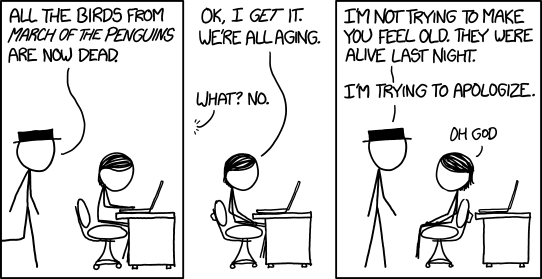
\includegraphics[width=4in]{march_of_the_penguins.png}
    \caption*{You ARE getting older, though}
\end{figure}

\end{document}
